\chapter{Implementacija i korisničko sučelje}
		
		
		\section{Korištene tehnologije i alati}
		
		Tim je komunicirao putem aplikacija WhatsApp\footnote{\url{https://www.whatsapp.com/}} te Discord\footnote{\url{https://discord.com/}}. WhatsApp je besplatna aplikacija za dopisivanje te je prvenstveno služila za međusobne dogovore kao i razrješavanje pojedinih nejasnoća. Discord je  aplikacija i platforma za digitalnu distribuciju, dizajnirana prvenstveno za zajednice koje se bave igranjem video igara. Specijalizirana je za tekstualnu, slikovnu, video i audio komunikaciju između korisnika što je uvelike olakšalo komunikaciju prilikom procesa izrade aplikacije. Za izradu UML dijagrama korišten je alat Astah Professional\footnote{\url{https://astah.net/products/astah-professional/}} te Visual Paradigm\footnote{\url{https://www.visual-paradigm.com/}}. Kao sustav za upavljanje izvornim kodom koristio se Git\footnote{\url{https://git-scm.com/}}, a udaljeni repozitorij projekta je dostupan na web platformi Gitlab\footnote{\url{https://gitlab.com/}}.
		\newline

Kao razvojna okruženja korišteni su IntelliJ IDEA\footnote{\url{https://www.jetbrains.com/idea/}}, Eclipse\footnote{\url{https://www.eclipse.org/}} te Microsoft Visual Studio\footnote{\url{https://visualstudio.microsoft.com/}}. IntelliJ IDEA je integrirano razvojno okruženje (IDE) napisano u Javi za razvoj računalnog softvera napisanog u Javi, Kotlinu, Groovyju i drugim jezicima koji se temelje na JVM-u. Razvio ga je JetBrains (ranije poznat kao IntelliJ) i dostupan je kao Apache 2 licencirano izdanje zajednice i u vlasničkom komercijalnom izdanju. Oba se izdanja mogu koristiti za komercijalni razvoj. Eclipse je integrirano razvojno okruženje koje se koristi u računalnom programiranju. Sadrži osnovni radni prostor i proširivi sustav za prilagođavanje okruženja. To je drugi najpopularniji IDE za Java razvoj, a do 2016. bilo je najpopularniji. Visual Studio je integrirano razvojno okruženje tvrtke Microsoft. Koristi se za razvoj računalnih programa uključujući web stranice, web aplikacije, web usluge i mobilne aplikacije.
		\newline

Aplikacija je napisana pomoću radnog okvira Spring framework\footnote{\url{https://spring.io/projects/spring-framework}} i jezika Java\footnote{\url{https://www.java.com/en/}} za izradu \textit{backenda}, a za izradu \textit{frontenda} koristio se React\footnote{\url{https://reactjs.org/}} te jezik Javascript\footnote{\url{https://www.javascript.com/}}. Spring framework omogućava jednostavan razvoj modernih aplikacija u Javi. Nudi brojne značajke koje su organizirane u module. Središnji modul je Spring spremnik čija je dužnost povezivanje, konfiguriranje, stvaranje i upravljanje životnim ciklusom pojedinog objekta, tj. Spring bean-a. Za razvoj web aplikacija veliku važnost ima Spring MVC modul. On kombinira sve prednosti \textit{Model-View-Controller} obrasca i Spring okvira. Osim Spring modula postoje i Spring projekti, a oni nude sve značajke za određenu funkcionalnost. React je Javascript biblioteka otvorenog koda koja se temelji na lakšem dizajniranju sučelja. Odgovoran je za prikaz slojeva u aplikaciji, a napravio ga je Facebook. React omogućuje programiranje i razvoj aplikacija te je važan dio za  \textit{frontend} development.
	\newline

Za razvoj i testiranje HTTP REST API-ja korišten je alat Postman\footnote{\url{https://www.postman.com/}}, a baza podataka se prije procesa \textit{deploymenta} nalazila lokalno što je ostvareno pomoću PostgreSQL-a\footnote{\url{https://www.postgresql.org/}}, sustava za upravljanje relacijskom bazom podataka otvorenog koda. Nakon \textit{deploymenta} baza podataka se nalazi na poslužitelju u oblaku Render\footnote{\url{https://render.com/}}.
			
			\eject 
		
	
		\section{Ispitivanje programskog rješenja}
			
	
			
			\subsection{Ispitivanje komponenti}

   
			\textbf{Ispitni slučaj 1: Login sa postojećim i nepostojećim korisnikom, te korisnikom čija konferencija više nije dostupna. }
   
   \textbf{Ulaz:}
   \begin{packed_item}
   \item[] \begin{packed_enum}
				
				\item Username i password postojećeg korisnika
    \item Username i password nepostojećeg korisnika
    \item Username i password korisnika čija konferencije više nije dostupna
				
			\end{packed_enum}
   \end{packed_item}

   \textbf{Očekivani rezultat:}
   \begin{packed_item}
   \item[] \begin{packed_enum}
				
				\item Login je uspješan za postojećeg korisnika i kao odgovor se vraća korisnički račun usera.
    \item Login je neuspješan za nepostojećeg korisnika i kao odgovor se vraća Unauthorised.
    \item Login je neuspješan za korisnika čija je konferencija nedostupna i odgovor je Forbidden.
				
			\end{packed_enum}
   \end{packed_item}
   \textbf{Rezultat:} \text Svaki očekivani rezultat je ostvaren. \color{red} Aplikacija je prošla test. \color{black}

    \begin{figure}[H]
            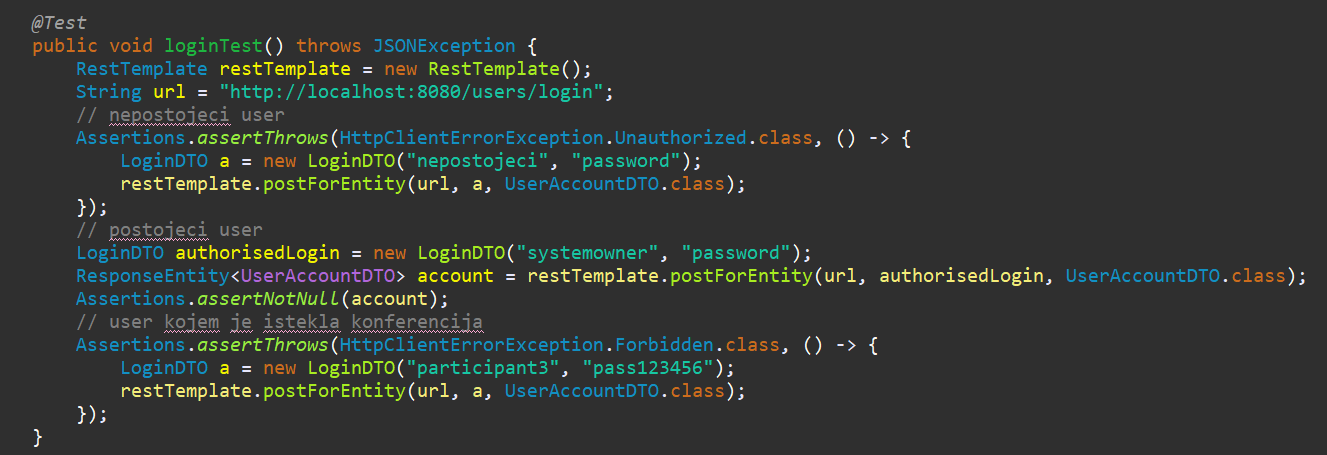
\includegraphics[scale=0.55]{slike/login.png} %veličina
			
			\centering
			\caption{Testiranje prijave}
			\label{fig:testiranje prijave}
			\end{figure}






   \textbf{\newline Ispitni slučaj 2: Registracija korisnika\newline  }
   \textbf{Ulaz:}
   \begin{packed_item}
   \item[] \begin{packed_enum}
				
				\item Stvaranje konferencije te unos ispravnih podataka o korisniku.
    \item Stvaranje konferencije, te unos neispravnih podataka za korisnika (neispravni format e-maila, neispravan format broja mobitela, nedovoljan broj znakova za username, nedovoljan broj znakova za password itd.).
				
			\end{packed_enum}
   \end{packed_item}

   \textbf{Očekivani rezultat:}
   \begin{packed_item}
   \item[] \begin{packed_enum}
				
				\item Registracija je uspješna i kao odgovor se vraća stvoreni korisnički račun.
    \item Registracija je neuspješna te se kao odgovor vraća BadRequest.
				
			\end{packed_enum}
   \end{packed_item}
   \textbf{Rezultat:} \text Svaki očekivani rezultat je ostvaren. \color{red} Aplikacija je prošla test. \color{black}

    \begin{figure}[H]
            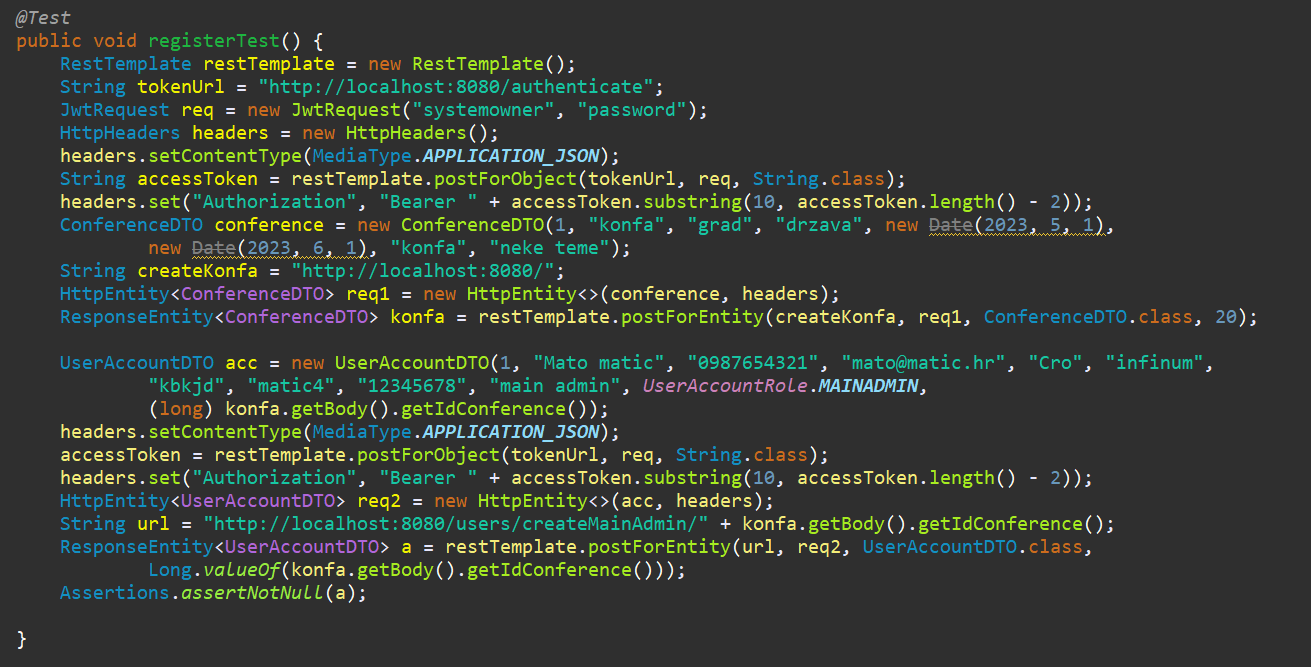
\includegraphics[scale=0.55]{slike/register_test.png} %veličina
			
			\centering
			\caption{Test ispravne registracije korisnika}
			\label{fig:ispravna registracija test}
			\end{figure}

    \begin{figure}[H]
            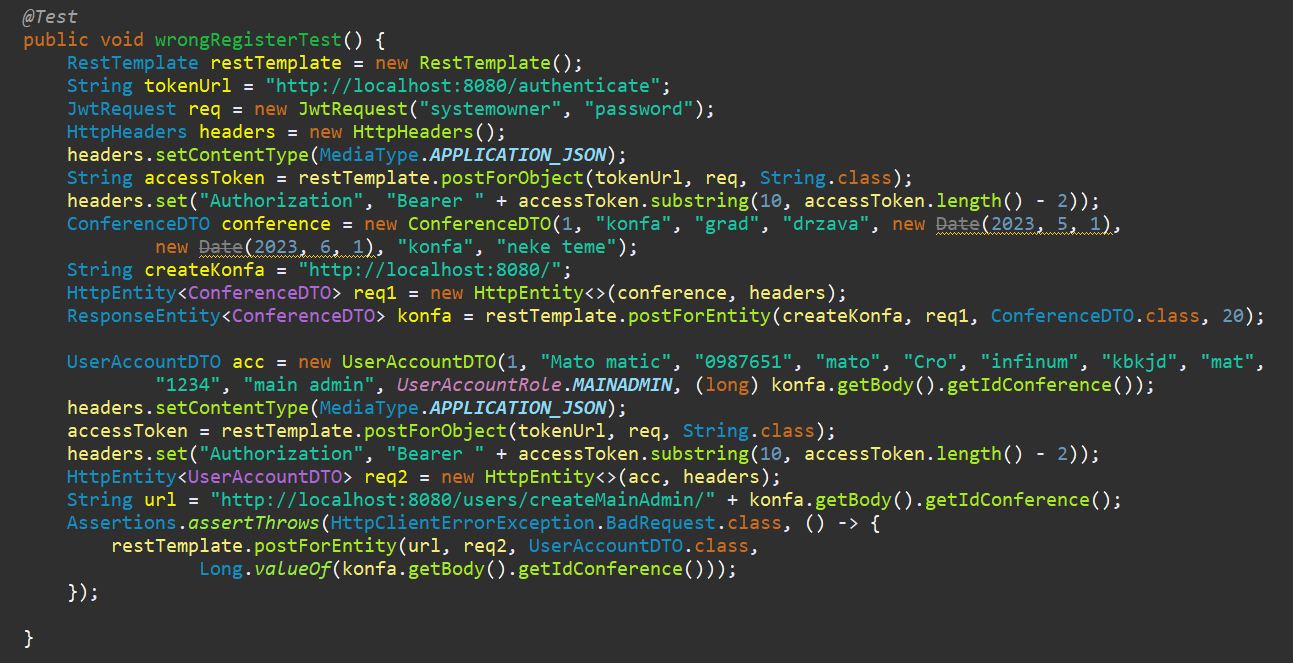
\includegraphics[scale=0.55]{slike/wrong_register_test.png} %veličina
			
			\centering
			\caption{Neispravna registracija korisnika}
			\label{fig:neispravna registracija korisnika}
			\end{figure}
  



   \textbf{\newline Ispitni slučaj 3: Kreiranje konferencije \newline}
   \textbf{Ulaz:}
   \begin{packed_item}
   \item[] \begin{packed_enum}
				
				\item Stvaranje konferencije sa svim ispravnim podatcima.
    \item Kreiranje konferencije s neispravnim podatcima (npr. datum početka je nakon datuma završetka).
				
			\end{packed_enum}
   \end{packed_item}

   \textbf{Očekivani rezultat:}
   \begin{packed_item}
   \item[] \begin{packed_enum}
				
				\item Kreiranje konferencije je uspješno. Kao odgovor se vraća kreirana konferencija.
    \item Kreiranje konferencije je neuspješno i kao odgovor se vraća BadRequest.
				
			\end{packed_enum}
   \end{packed_item}
   \textbf{Rezultat:} \text Svaki očekivani rezultat je ostvaren. \color{red} Aplikacija je prošla test. \color{black}

    \begin{figure}[H]
            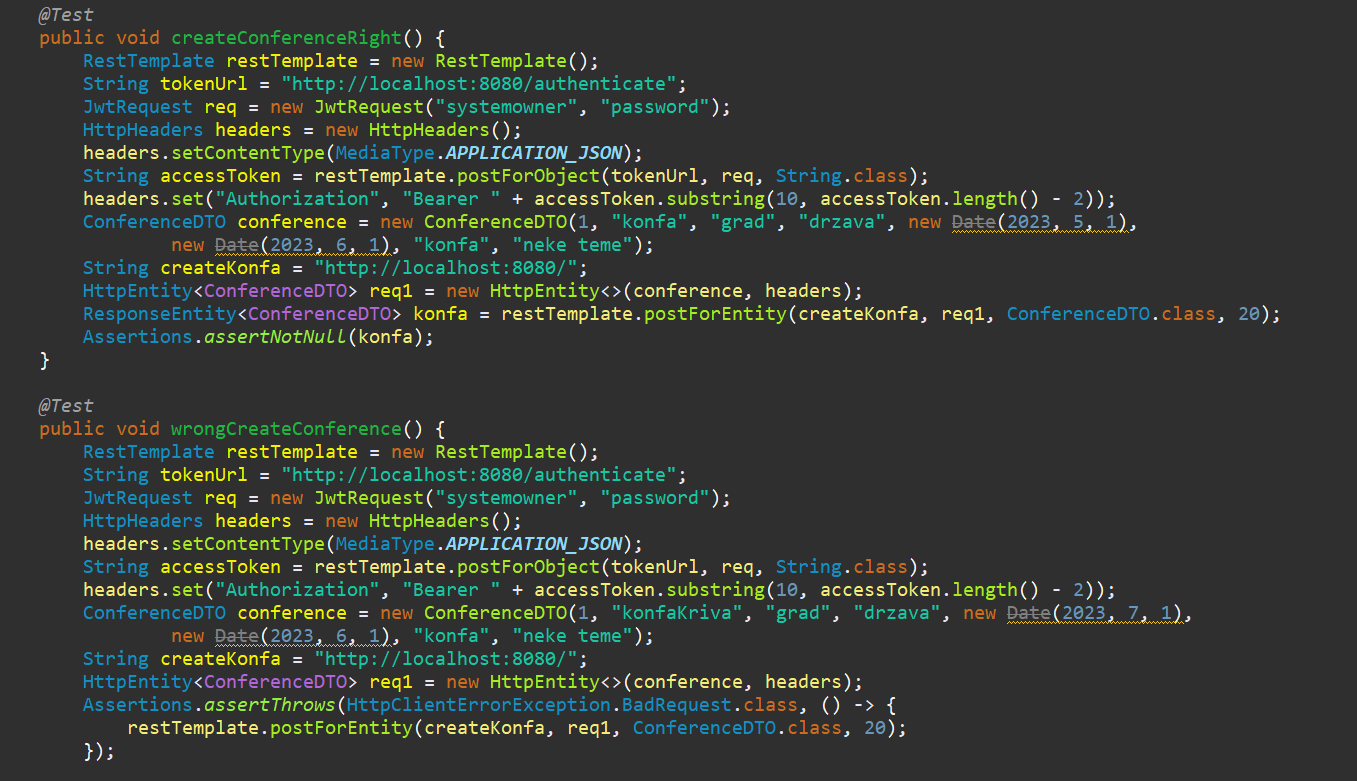
\includegraphics[scale=0.55]{slike/conf_test.png} %veličina
			
			\centering
			\caption{Testiranje kreiranja konferencije}
			\label{fig:test kreiranja konferencije}
			\end{figure}

   
   			\textbf{Ispitni slučaj 4: Stvaranje grupe podataka \newline}
   
   \textbf{Ulaz:}
   \begin{packed_item}
   \item[] \begin{packed_enum}
				
				\item Podatci o grupi podataka koju pokušava stvoriti ovlašteni glavni admin.
    \item Podatci o grupi podataka koju pokušava stvoriti neovlašteni operativni admin.
				
			\end{packed_enum}
   \end{packed_item}

   \textbf{Očekivani rezultat:}
   \begin{packed_item}
   \item[] \begin{packed_enum}
				
				\item Kreiranje grupe podataka je uspješno i kao odgovor se vraća stvorena grupa podataka.
    \item  Kreiranje grupe podataka je neuspješno i kao odgovor se vraća Forbidden.
				
			\end{packed_enum}
   \end{packed_item}
   \textbf{Rezultat:} \text Svaki očekivani rezultat je ostvaren. \color{red} Aplikacija je prošla test. \color{black}

    \begin{figure}[H]
            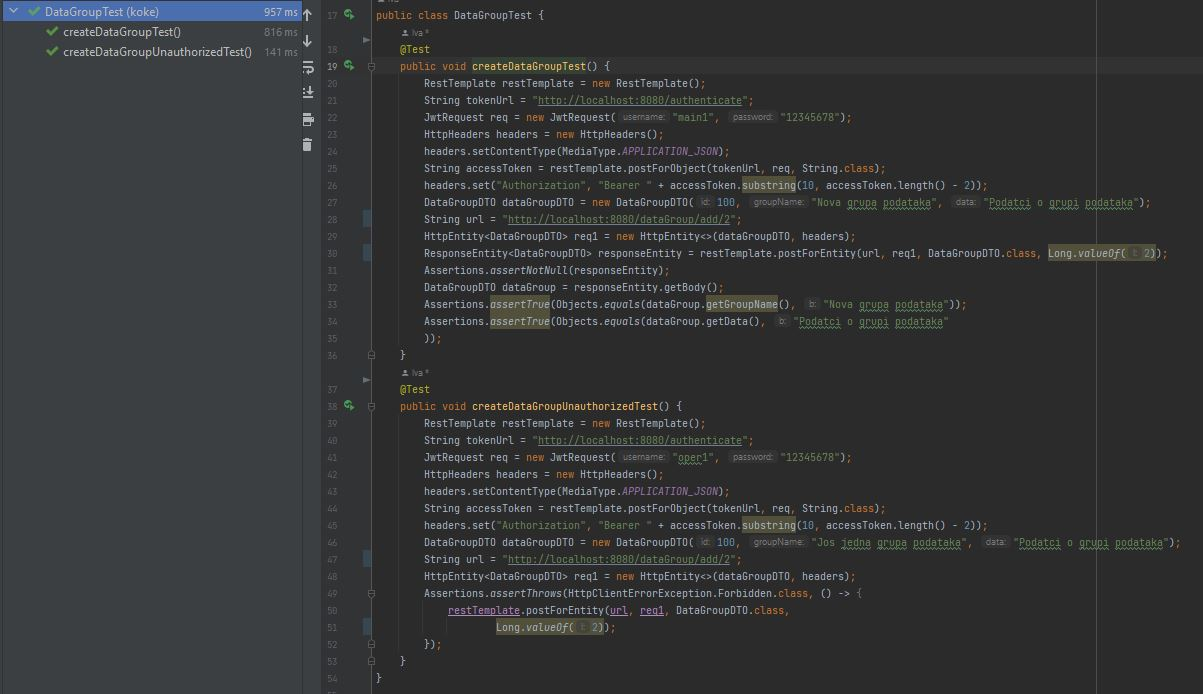
\includegraphics[scale=0.55]{slike/DataGroupTest.JPG} %veličina
			
			\centering
			\caption{Testiranje kreiranja grupe podataka}
			\label{fig:testiranje kreiranja grupe podataka}
			\end{figure}

   
   			\textbf{Ispitni slučaj 5: Stvaranje specijalnog događaja za konferenciju \newline}
   
   \textbf{Ulaz:}
   \begin{packed_item}
   \item[] \begin{packed_enum}
				
				\item Podatci o specijalnom događaju kojeg pokušava stvoriti ovlašteni glavni admin.
    \item Podatci o specijalnom događaju kojeg pokušava stvoriti neovlašteni operativni admin.
				
			\end{packed_enum}
   \end{packed_item}

   \textbf{Očekivani rezultat:}
   \begin{packed_item}
   \item[] \begin{packed_enum}
				
				\item Kreiranje specijalnog događaja je uspješno i kao odgovor se vraća stvoreni specijalni događaj.
    \item  Kreiranje specijalnog događaja je neuspješno i kao odgovor se vraća Forbidden.
				
			\end{packed_enum}
   \end{packed_item}
   \textbf{Rezultat:} \text Svaki očekivani rezultat je ostvaren. \color{red} Aplikacija je prošla test. \color{black}

    \begin{figure}[H]
            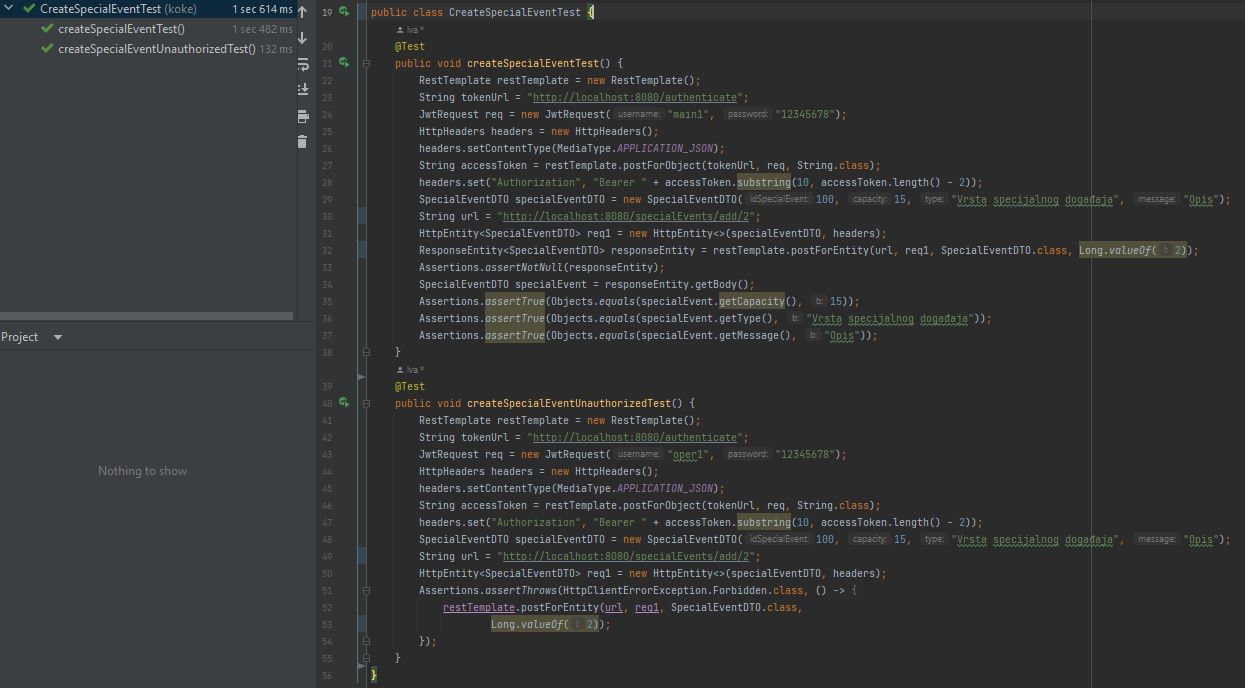
\includegraphics[scale=0.55]{slike/CreateSpecialEventTest.JPG} %veličina
			
			\centering
			\caption{Testiranje kreiranja specijalnog događaja}
			\label{fig:testiranje kreiranja specijalnog događaja}
			\end{figure}

   
   			\textbf{Ispitni slučaj 6: Prijava sudionika na specijalni događaj \newline}
   
   \textbf{Ulaz:}
   \begin{packed_item}
   \item[] \begin{packed_enum}
				
				\item Sudionik se prijavljuje na događaj kojem kapacitet nije popunjen.
    \item Sudionik se prijavljuje na događaj kojem kapacitet je popunjen.
				
			\end{packed_enum}
   \end{packed_item}

   \textbf{Očekivani rezultat:}
   \begin{packed_item}
   \item[] \begin{packed_enum}
				
				\item Sudionik se uspješno prijavio na događaj i kao odgovor se vraća taj  specijalni događaj.
    \item  Sudionik se nije prijavio na događaj, već je dodan u listu čekanja za taj događaj i na njegov email mu dolazi obavijest, a ovlaštenom glavnom adminu šalje se mail da lista čekanja nije prazna te da, ako je moguće, poveća kapacitet. Kao odgovor se vraća isti specijalni događaj.
				
			\end{packed_enum}
   \end{packed_item}
   \textbf{Rezultat:} \text Svaki očekivani rezultat je ostvaren. \color{red} Aplikacija je prošla test. \color{black}

    \begin{figure}[H]
            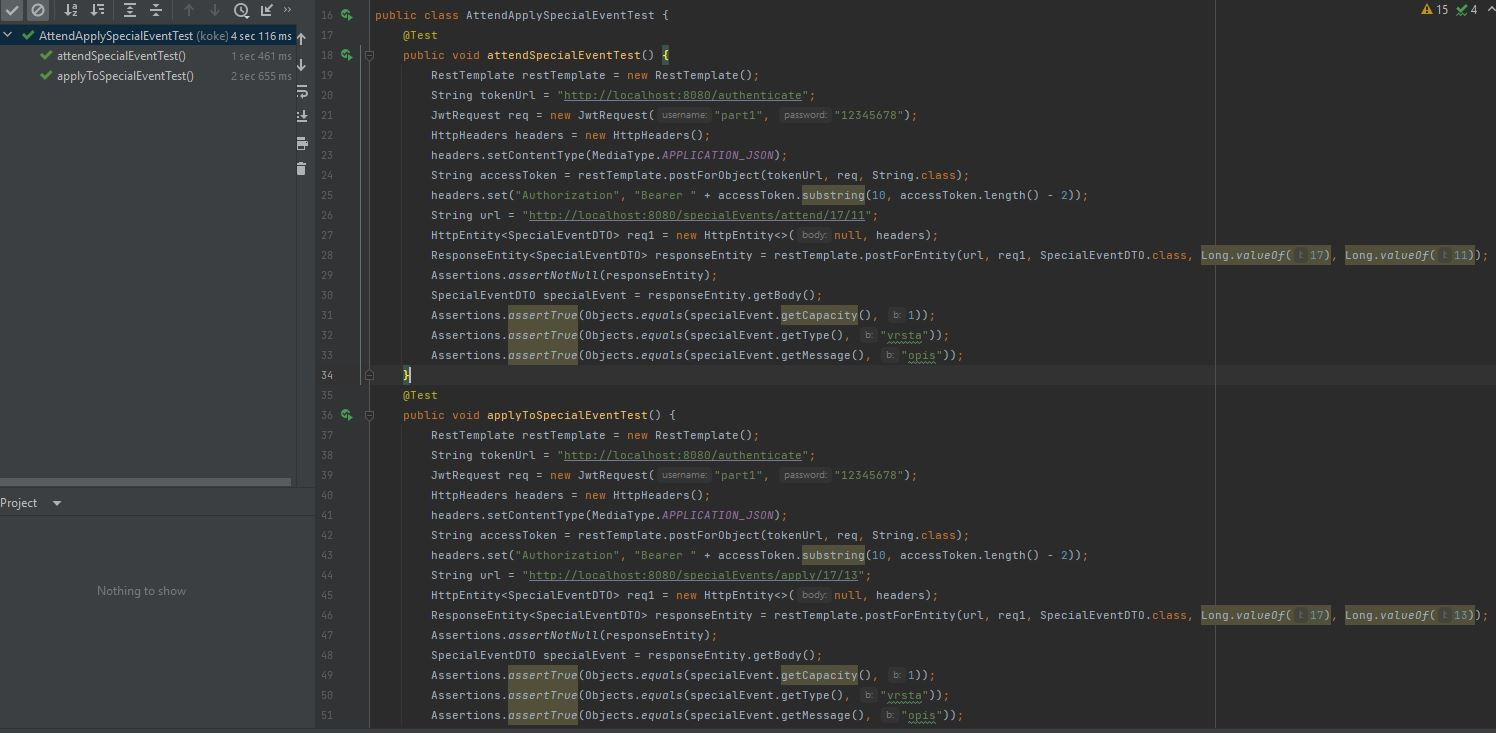
\includegraphics[scale=0.45]{slike/ApplyAttendSpecialEventTest.JPG} %veličina
			
			\centering
			\caption{Testiranje prijave na specijalni događaj}
			\label{fig:testiranje prijave na specijalni događaj}
			\end{figure}

   
   
   			\textbf{Ispitni slučaj 7: Povećanje kapaciteta specijalnog događaja \newline}
   
   \textbf{Ulaz:}
   \begin{packed_item}
   \item[] \begin{packed_enum}
				
				\item Ovlašteni glavni admin unosi za koliko želi povećati kapacitet specijalnog događaja.
				
			\end{packed_enum}
   \end{packed_item}

   \textbf{Očekivani rezultat:}
   \begin{packed_item}
   \item[] \begin{packed_enum}
				
				\item Kapacitet specijalnog događaja je povećan. Šalje se mail sudionicima na listi čekanja da su sada prijavljeni na specijalni događaj. Kao odgovor se vraća isti specijalni događaj.
				
			\end{packed_enum}
   \end{packed_item}
   \textbf{Rezultat:} \text Očekivani rezultat je ostvaren. \color{red} Aplikacija je prošla test. \color{black}

    \begin{figure}[H]
            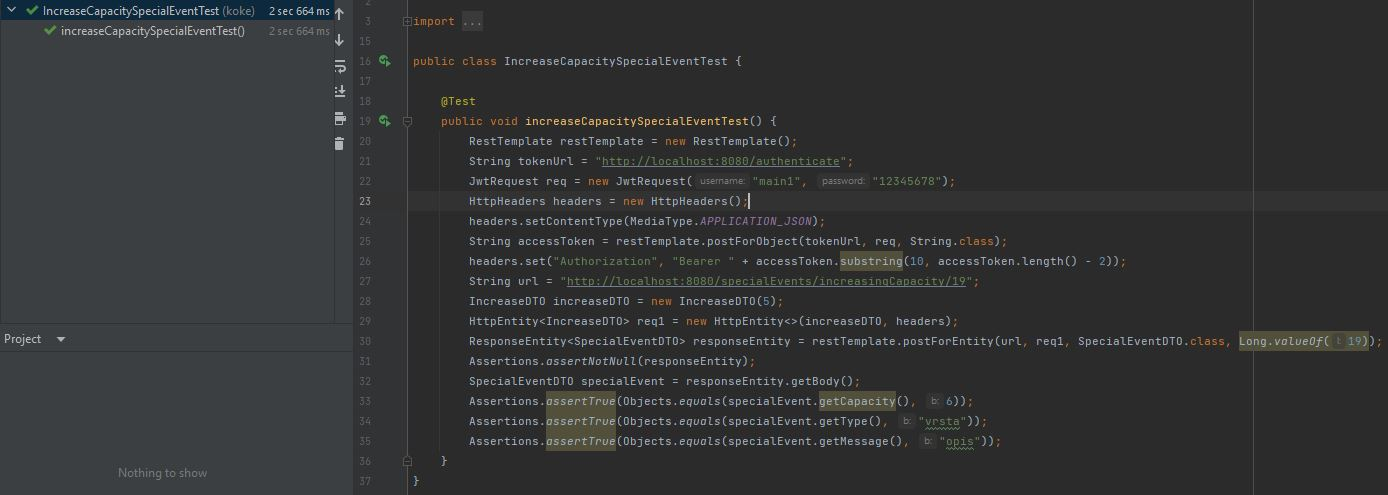
\includegraphics[scale=0.45]{slike/IncreaseCapacitySpecialEvent.JPG} %veličina
			
			\centering
			\caption{Testiranje povećanja kapaciteta specijalnog događaja}
			\label{fig:testiranje povećanja kapaciteta specijalnog događaja}
			\end{figure}

			
			\subsection{Ispitivanje sustava}
		\textbf{Ispitni slučaj 1: Uspješan login s postojećim korisnikom\newline}

  \newLine
   
   \textbf{Ulaz:}
   \begin{packed_item}
   \item[] \begin{packed_enum}
				
				\item Korisničko ime i lozinka postojećeg korisnika
				
			\end{packed_enum}
   \end{packed_item}

   \textbf{Očekivani rezultat:}
   \begin{packed_item}
   \item[] \begin{packed_enum}
				
				\item Login je uspješan i preusmjerava nas na početni izbornik. 
				
			\end{packed_enum}
   \end{packed_item}
   \textbf{Rezultat:} \text Očekivani rezultat je ostvaren. \color{red} Aplikacija je prošla test. \color{black}

    \begin{figure}[H]
            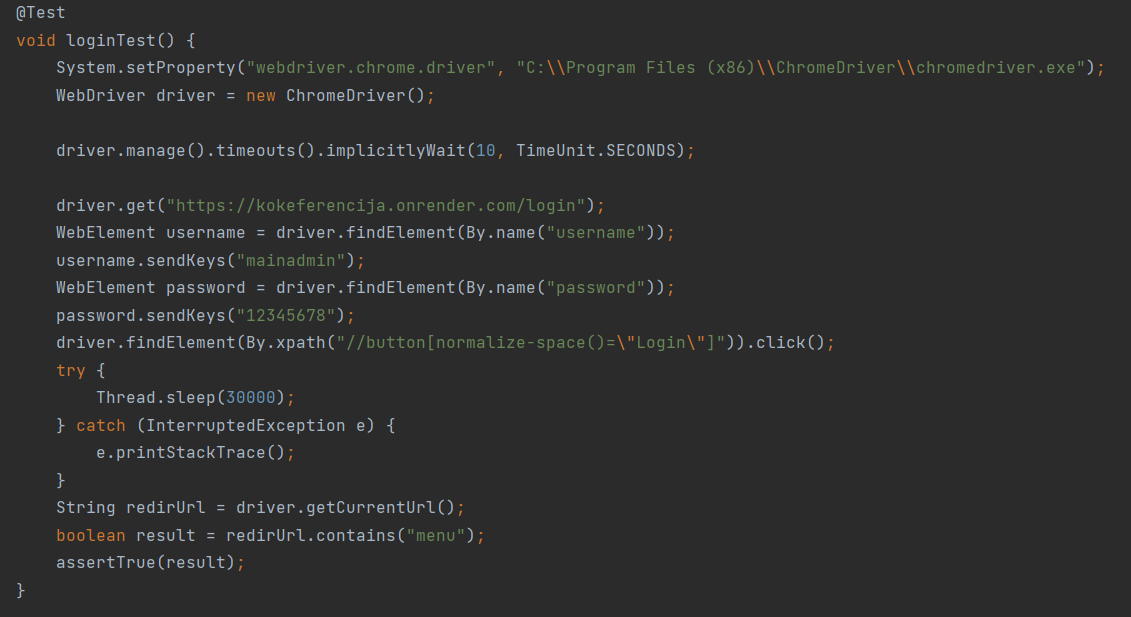
\includegraphics[width = \textwidth]{slike/Login succesful.png}
			
			\centering
			\caption{Uspješan login - Selenium}
			\label{fig:uspjesan login selenium}
			\end{figure}

   \textbf{Ispitni slučaj 2: Neuspješan login s nepostojećim korisnikom\newline}

  \newLine
   
   \textbf{Ulaz:}
   \begin{packed_item}
   \item[] \begin{packed_enum}
				
				\item Korisničko ime i lozinka nepostojećeg korisnika
				
			\end{packed_enum}
   \end{packed_item}

   \textbf{Očekivani rezultat:}
   \begin{packed_item}
   \item[] \begin{packed_enum}
				
				\item Login je neuspješan i ne preusmjerava nas na početni izbornik. 
				
			\end{packed_enum}
   \end{packed_item}
   \textbf{Rezultat:} \text Očekivani rezultat je ostvaren. \color{red} Aplikacija je prošla test. \color{black}

    \begin{figure}[H]
            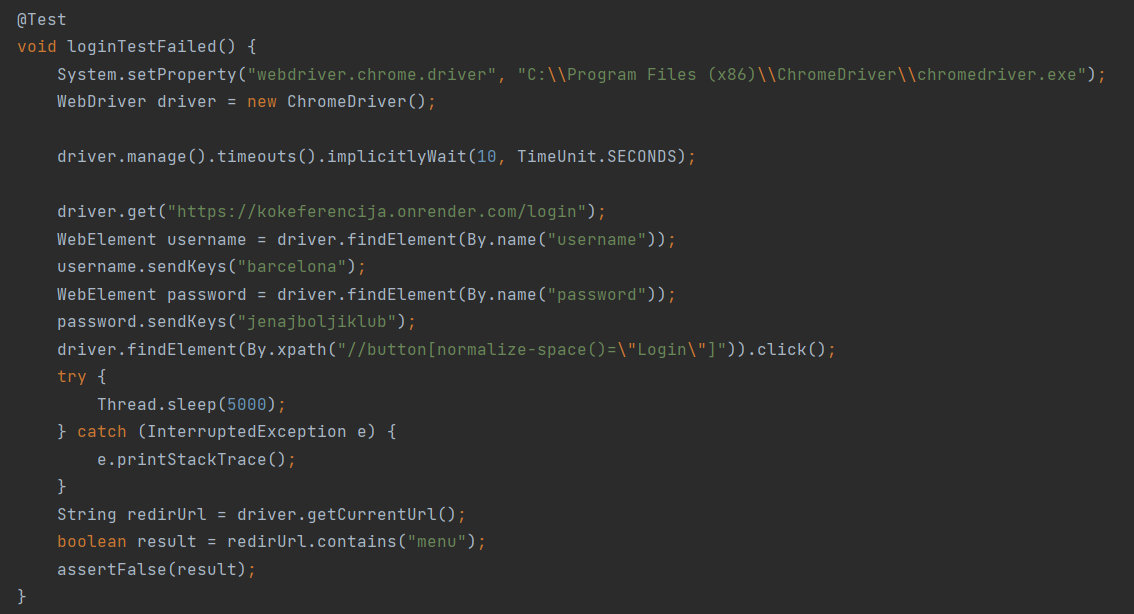
\includegraphics[width = \textwidth]{slike/login failed.png}
			
			\centering
			\caption{Neuspješan login - Selenium}
			\label{fig:neuspjesan login selenium}
			\end{figure}

   \eject

   \textbf{Ispitni slučaj 3: Otvaranje stranice MyConference\newline}

  \newLine
   
   \textbf{Ulaz:}
   \begin{packed_item}
            \item Korisničko ime i lozinka postojećeg korisnika
   \end{packed_item}

   \textbf{Očekivani rezultat:}
   \begin{packed_item}
   \item[] \begin{packed_enum}
				
				\item Uspješno se dohvaćaju svi resursi za prikaz stranice MyConference i stranica se uspješno prikazuje. 
				
			\end{packed_enum}
   \end{packed_item}
   \textbf{Rezultat:} \text Očekivani rezultat je ostvaren. \color{red} Aplikacija je prošla test. \color{black}

    \begin{figure}[H]
            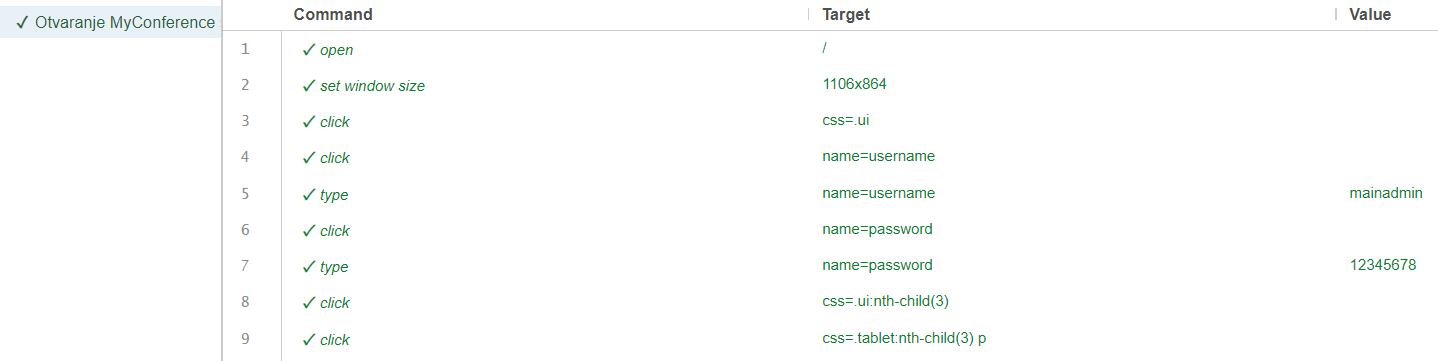
\includegraphics[width = \textwidth]{slike/MyConferenceTest.png}
			
			\centering
			\caption{Otvaranje MyConference test}
			\label{fig:myConferenceTest}
			\end{figure}

   \begin{figure}[H]
            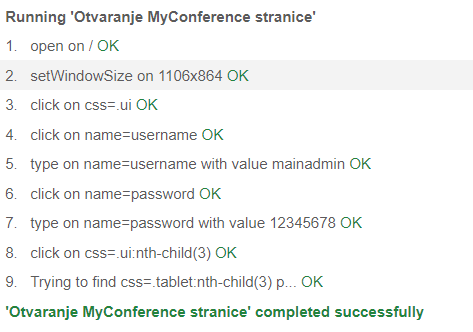
\includegraphics[scale = 0.8]{slike/MyConferenceRez.png}
			
			\centering
			\caption{Otvaranje MyConference rezultat}
			\label{fig:myConferenceRez}
			\end{figure}

   \textbf{Ispitni slučaj 4: Otvaranje galerije\newline}

  \newLine
   
   \textbf{Ulaz:}
   \begin{packed_item}
            \item Korisničko ime i lozinka postojećeg korisnika
   \end{packed_item}

   \textbf{Očekivani rezultat:}
   \begin{packed_item}
   \item[] \begin{packed_enum}
				
				\item Uspješno se dohvaćaju svi resursi za prikaz galerije i stranica se uspješno prikazuje. 
				
			\end{packed_enum}
   \end{packed_item}
   \textbf{Rezultat:} \text Očekivani rezultat je ostvaren. \color{red} Aplikacija je prošla test. \color{black}

    \begin{figure}[H]
            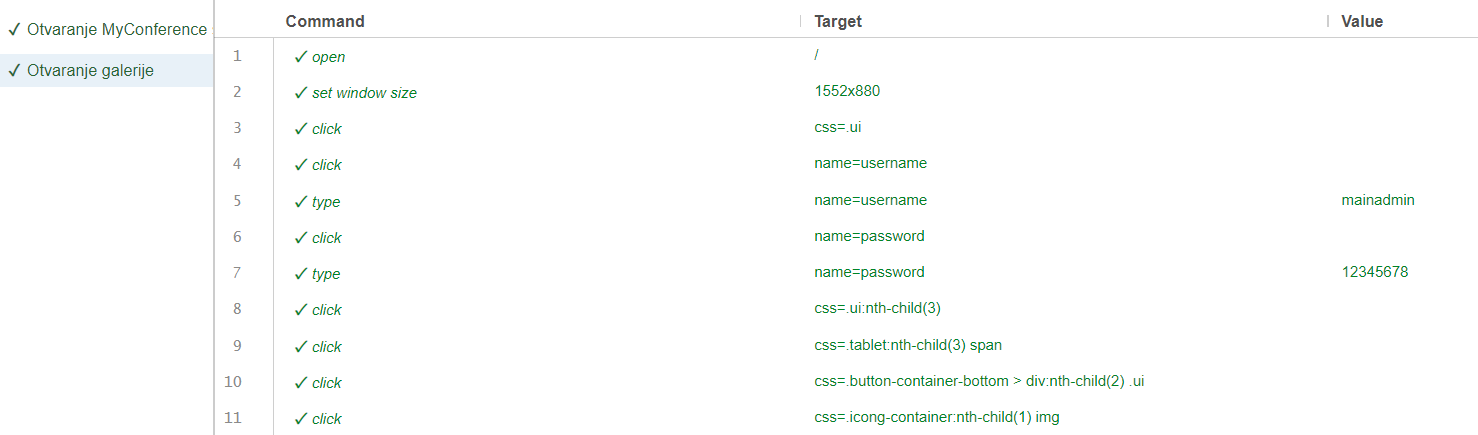
\includegraphics[width = \textwidth]{slike/OtvaranjeGalerije.png}
			
			\centering
			\caption{Otvaranje galerije test}
			\label{fig:myConferenceTest}
			\end{figure}

   \begin{figure}[H]
            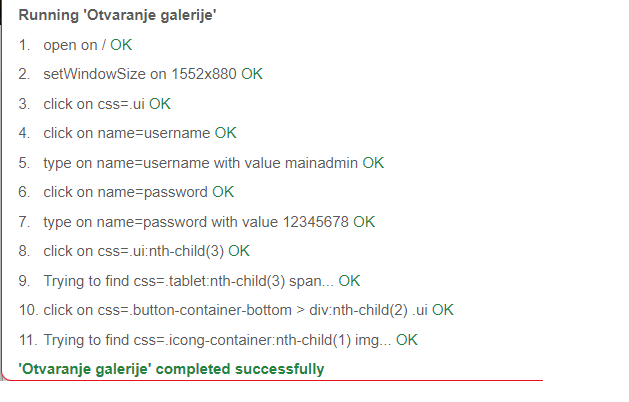
\includegraphics[scale = 0.8]{slike/OtvaranjeGalerijeRez.png}
			
			\centering
			\caption{Otvaranje galerije rezultat}
			\label{fig:myConferenceRez}
			\end{figure}
			
			\eject 
		
		
		\section{Dijagram razmještaja}
			
			Dijagram razmještaja opisuje topologiju sustava i usredotočen je na odnos
                sklopovskih i programskih dijelova. Arhitektura sustava aplikacije \textit{Kokeferencija} je ”klijent - poslužitelj” gdje se poslužitelj Render, na kojem se nalaze web stranica i baza podataka, nalazi na
                poslužiteljskom računalu, a klijenti koriste web preglednik kako bi pristupili web
                aplikaciji. Komunikacija između računala korisnika i poslužitelja odvija se preko 
                HTTP veze.

                \begin{figure}[H]
                 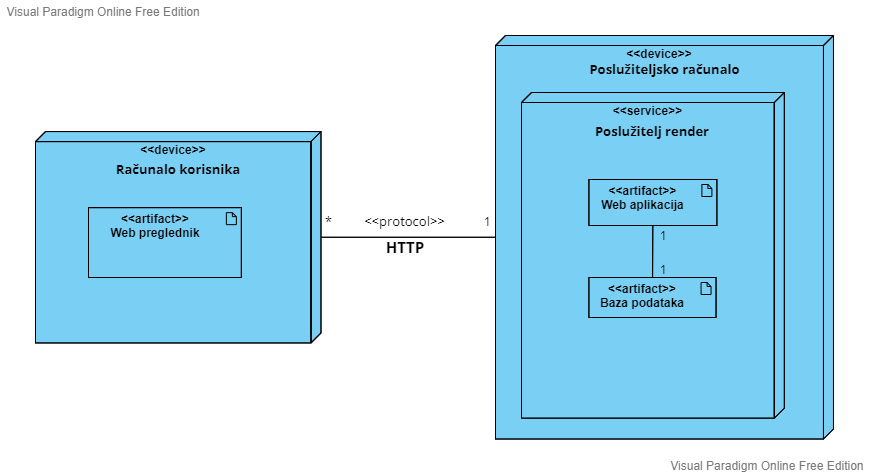
\includegraphics[scale = 0.55]{slike/dijagramRazmjestaja.png}
                \centering
                 \caption{dijagram razmještaja}
                 \label{fig:dijagram razmještaja}
                 \end{figure}\\

                 \eject


		
            \section{Upute za puštanje u pogon}

            \textbf{Postavljanje računa na Render\footnote{https://dashboard.render.com/}} \\
            Potrebno je stvoriti korisnički računa na Render-u, te 
           povezati ga s GitLab korisničkim računom kako bi mogli pristup projektu.\\
           \newLine

    \textbf{Konfiguracija i pokretanje poslužitelja baze podataka}\\
            Na nadzornoj ploči Rendera odabrati opciju New, zatim PostgreSQL. U polje \textit{Name} upisujemo ime baze koja se nalazi lokalno na našem računali, zatim u polja \textit{Database} i \textit{Username} opcionalno  upisujemo proizvoljno ime baze i korisničko ime. Za regiju odabiremo Frankfurt, te odgovarajuću PostegreSQL verziju. Za kraj odredimo besplatni plan. \\
            \newLine
             

            \textbf{Spajanje backend-a na poslužitelja baze podataka}\\
           U datoteku \textit{application.properties} upisujemo potrebne varijable. Kao \textit{spring.datasource.password} postavljamo lozinku koja se izgenerirala pri puštanju u pogon. Zatim postavljamo \textit{spring.datasource.username}. Url koji postavljamo ima oblik \textit{jdbc:postegreswl://hostname/database}. Za driver postavljamo \textit{org.postgresql.Driver}  Svi potrebi podatci o bazi koja je puštena u pogon nalaze se na Renderu(DashBoard 
            zatim naziv baze koji smo postavili pri pogonu). 
             U application.properties također dodamo liniju \textbf{server.servlet.context-path=/api} koja određuje prefiks svih zahtjeva na backend.
            \begin{figure}[H]
                 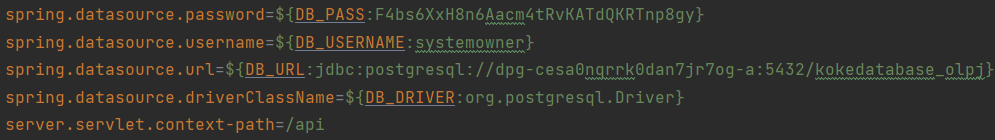
\includegraphics[width=\textwidth]{slike/application-properties.png}
                \centering
                 \caption{application.properties}
                 \label{fig:application.properties}
                 \end{figure}\\

        \textbf{Priprema backenda}\\
            Stvaramo Dockerfile u mapi u kojoj se nalazi \textit{sourcecode}. Konfiguracije datoteke jer prikazana na slici 5.10.
             \begin{figure}[H]
                 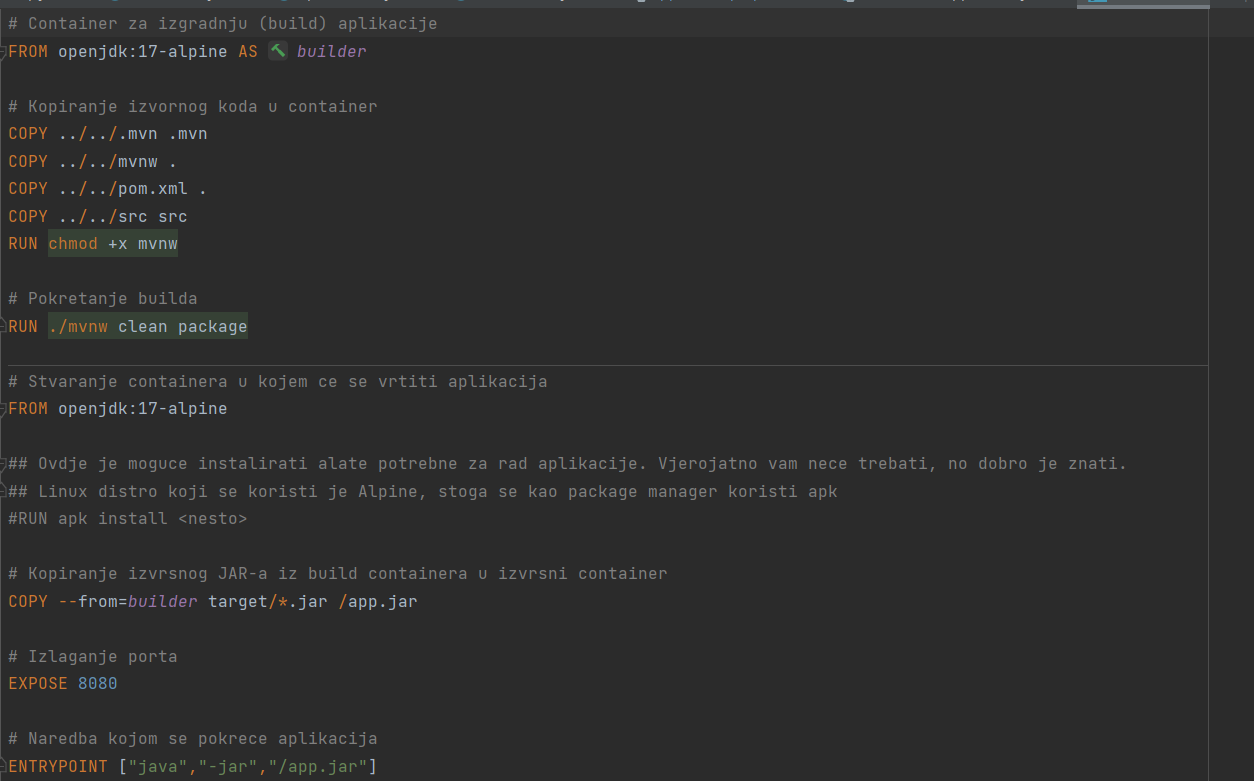
\includegraphics[scale = 0.5]{slike/Dockerfile.png}
                \centering
                 \caption{Dockerfile}
                 \label{fig:dockerfile}
                 \end{figure}\\\\

        \textbf{Puštanje backenda u pogon na Renderu}\\
            Na nadzornoj ploči Rendera izaberemo \textit{New} zatim \textit{Web Service}. Prikazat će se projekti povezanog GitLab računa. Pored odgovarajućeg projekta izaberemo \textit{Connect}. Postavljamo jedinstveno ime za servis (kokeferencije). Za regiju postavljamo Frankfurt. Zatim postavljamo granu na kojoj se nalazi kod i mapu u kojoj se nalazi izvorni kod. Za varijablu \textit{Environment} odabiremo \textit{Docker}.\\
            \begin{figure}[H]
                 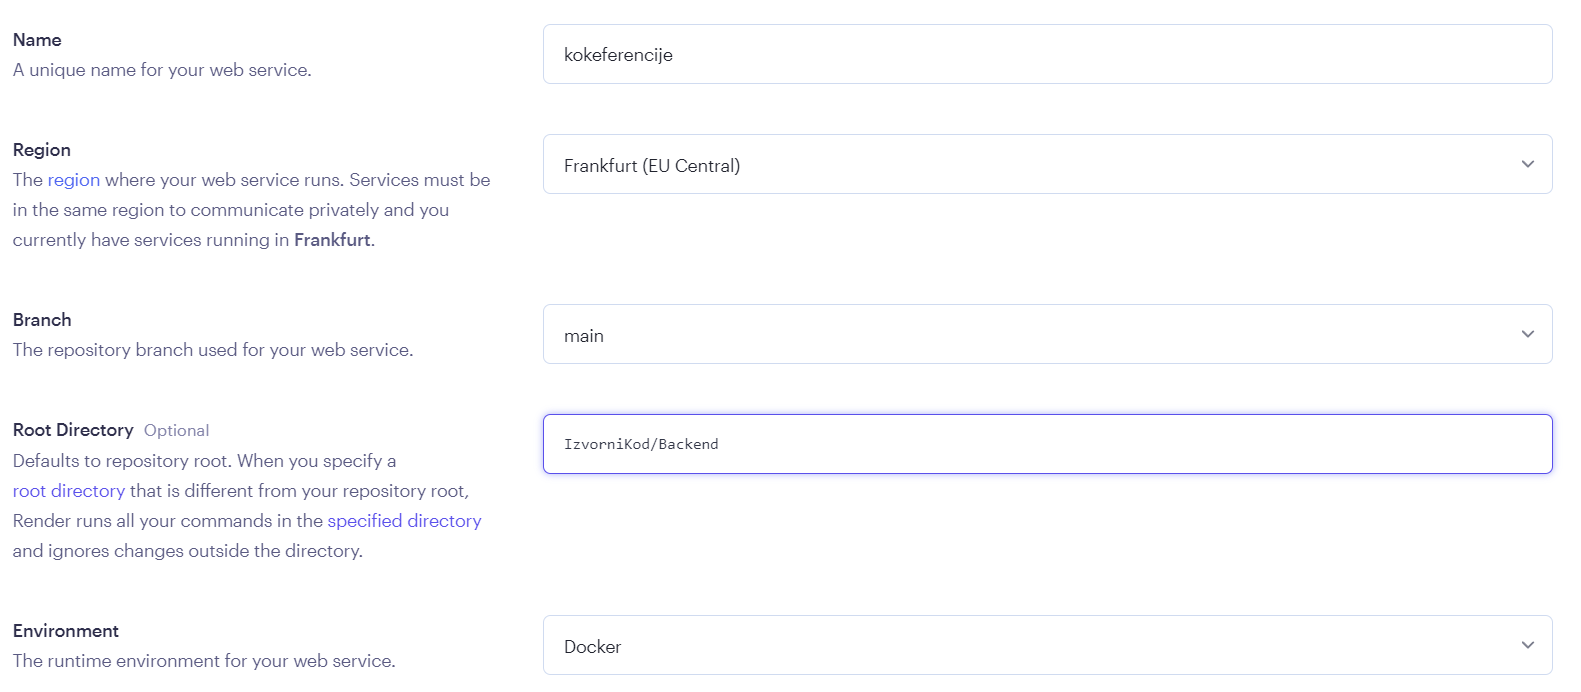
\includegraphics[width=\textwidth]{slike/Postavljanje backend za pogon.png}
                \centering
                 \caption{Postavljanje osnovnih varijabli za backend}
                 \label{fig:backend(1)}
                 \end{figure}
        Na dnu stranice odabiremo gumb \textit{Advanced}, zatim \textit{Add environment variable} te postavimo putanju za Dockerfile. Kada smo sve popunili odabiremo \textit{Create Web Service}.\\\\

        \textbf{Priprema frontenda}\\
        U package.json datoteku dodajemo ovisnosti potrebne za puštanje u pogon(http-proxy-middleware, dotenv, express)
         \begin{figure}[H]
                 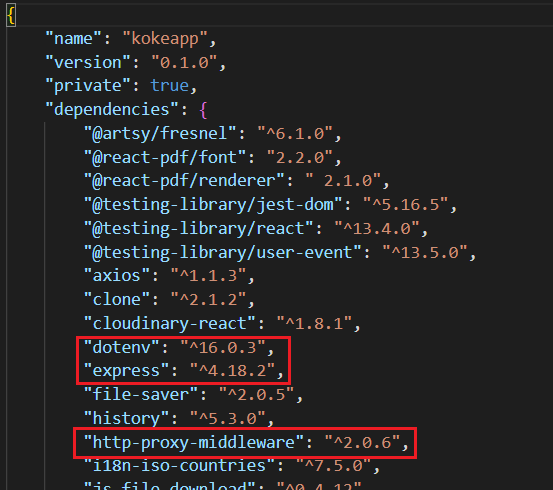
\includegraphics[scale = 0.70]{slike/package.json.png}
                \centering
                 \caption{package.json}
                 \label{fig:package.json}
                 \end{figure}
        U package.json izmijeniti naredbu \textbf{"build": "yarn install && react-scripts build"} i dodati naredbu \textbf{"start-prod": "node app.js"}.\\
        

        \textbf{Puštanje frontenda u pogon na Renderu}\\
             Na nadzornoj ploči Rendera izaberemo \textit{New} zatim \textit{Web Service}. Pored odgovarajućeg projekta odaberemo \textit{Connect}. Postavljamo ime za frontend servis koje će biti dio web-adrese (kokeferencija). Za regiju odabiremo Frankfurt, zatim odabiremo grane i mapu u kojoj se nalazi kod. Za varijablu \textit{Environment} biramo \textit{Node}. Za naredbu \textit{Build Command} postavljamo \textbf{yarn build}, a za \textit{Start Command} postavljamo \textbf{yarn start-prod}. Na dnu stranice odabiremo gumb \textit{Advanced} zatim \textit{Add Environment Variable}. Kao ključ postavljamo \textbf{APIBASEURL} a vrijednost postavljamo na adresu backend-a koji je pušten u pogon. Pritisnemo \textit{Create Web Service}. \\
        \textbf{Pokretanje web-stranice}\\
            Aplikaciji se može pristupiti preko adrese \textit{ https://kokeferencija.onrender.com/ \footnote{https://kokeferencija.onrender.com/}}.

    \eject 